\begin{minipage}[l]{0.5\textwidth}
  \begin{exerciseS}[Lamina inclinata]
 Un getto di acqua ($\rho = 1000 \ kg/m^3$) colpisce una lamina
 di massa per unità di apertura $m = 1 \ kg/m$ inclinata di un 
 angolo $\alpha = 30\degree$ rispetto all'orizzontale, connessa a terra
 con una molla di costante elastica $k = 10^5 \ N/m^2$. 
 Il getto esce con profilo uniforme $U=10 \ m/s$ da una fessura
 larga $d_1 = 5 \ cm$
 Determinare:
 \begin{itemize}
   \item la velocità $U_2$ (uniforme) e lo spessore $d_2$ del getto
     alla quota $H=1 \ m$ sopra la fessura di uscita, supponendo 
     trascurabili ogni forma di dissipazione e la curvatura delle 
     linee di corrente;
   \item la velocità massima $V$ del profilo triangolare di spessore
     $h = 2 \ cm$, identico su entrambe le estremità della lamina;
   \item la deformazione della molla, considerando trascurabili gli 
     sforzi viscosi all'interfaccia tra il getto e l'atmosfera 
     circostante ($P_a = 101325 \ Pa$) e la
     gravità agente sul fluido al di sopra della quota $H$.
 \end{itemize}
 \end{exerciseS}

\end{minipage}
\hspace{3mm}
\begin{minipage}[r]{0.5\textwidth}
 \centering
  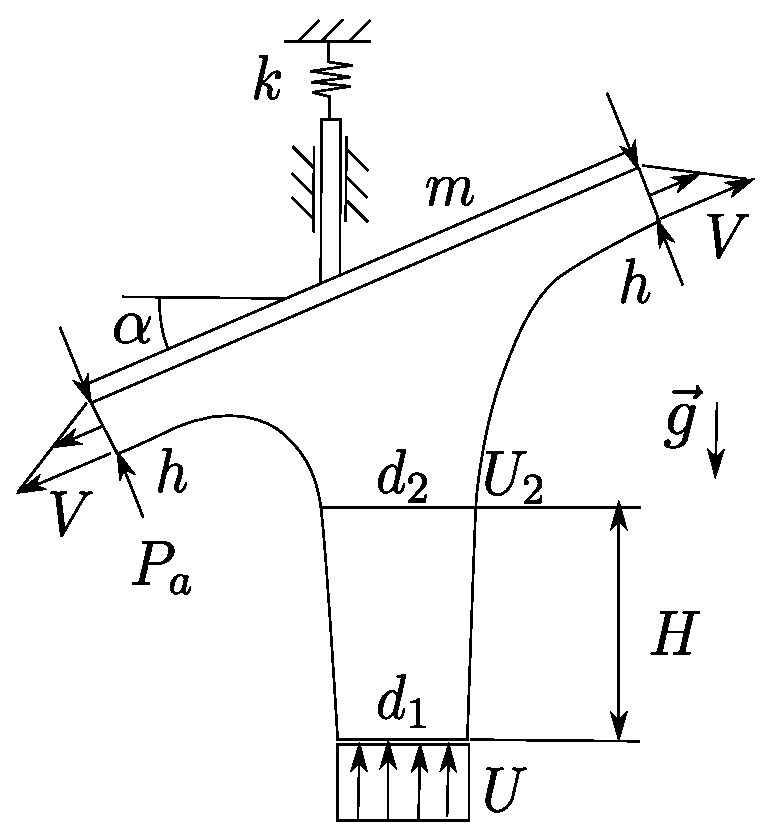
\includegraphics[width=1.0\textwidth]{./fig/jet_angle}
\end{minipage}

\sol

\partone
 Teorema di Bernoulli nell'ipotesi di stazionarietà, fluido incomprimibile, non viscoso, irrotazionale. Bilanci integrali.
 
\parttwo
\begin{itemize}
  \item continuità + Bernoulli
    \begin{equation}
      \begin{cases}
        \rho d U = \rho d_2 U_2 \\
        \frac{1}{2} \rho U^2 = \frac{1}{2} \rho U_2^2 + \rho g H
      \end{cases}
      \qquad \Rightarrow \qquad
      \begin{cases}
        d_2 = d_1 \left( 1 - \dfrac{2 g H}{U^2} \right)^{-1/2} = 0.0558 \ m \\
        U_2 = U \left( 1 - \dfrac{2 g H}{U^2} \right)^{1/2} = 8.96 \ m/s \\
      \end{cases}
    \end{equation}
  \item continuità: in ingresso profilo uniforme, in uscita due profili triangolari.
    \begin{equation}
      U d_1 = 2 \dfrac{1}{2} V h \Rightarrow V = U \dfrac{d_1}{h} = 25 \ m/s
    \end{equation}
  \item  bilancio di massa + equilibrio corpo: pressione $P_a$ ovunque; 
  i due flussi di quantità di moto sulla lamina si bilanciano: rimane 
  solo il termine in ingresso  
    \begin{equation}
    \bm{R}_{fl} = - \oint_{\partial \Omega} \rho \bm{u} \bm{u}
    \cdot \bm{\hat{n}}  =  \dots  = \rho U^2 \dfrac{d_1^2}{d_2} \bm{\hat{y}} = 4482.7 \ N \bm{\hat{y}}
    \end{equation}
    \begin{equation}
      k \Delta x = m g - R \Rightarrow \Delta x = - 0.0447 \ m \ \text{(compressione)}
    \end{equation}
\end{itemize}





